\documentclass{article}

\usepackage[utf8]{inputenc}
\usepackage[T1]{fontenc}
\usepackage{lipsum}
\usepackage{graphicx}
\usepackage{amsmath}
\usepackage[margin=1in]{geometry}
\usepackage{titlesec}
\usepackage{parskip}
\usepackage{tcolorbox}

\titleformat{\section}
{\LARGE\bfseries}{\thesection}{1em}{}

\titleformat{\subsection}
{\Large\bfseries}{\thesection}{1em}{}

\begin{document}

\pagestyle{empty}

\section*{Rust}
\large

Rust è un linguaggio di sistema (come C/C++, il compilato può girare sul bare metal, senza il supporto di un sistema operativo).

Nasce all'interno della Mozilla foundation, con forti influenze da OCaml e C++. Proprio in OCaml viene scritto il suo primo compilatore, anche se ora il codice viene compilato in Rust stesso (con LLVM come backend).

Come tutti i linguaggi a livello di sistema \textbf{non è presente un runtime} (in realtà è presente un runtime minimo), infatti non utilizza system threads e non ha un garbage collector.

Inoltre, è presente una \textbf{zero-cost abstraction}, con polimorfismo parametrico via monomorfizzazione. Il complesso sistema di ownership dei dati in memoria è interamente imposto a compile-time.

Viene garantita la \textbf{memory safety}, non avendo memory leaks, double deallocation, dangling pointes e data races.

Per concludere, è presente un sistema di \textbf{fearless concurrency}, dove il type system (insieme agli smart pointers) minimizzano i problemi legati alla concorrenza.

Sono inoltre presenti anche alcune features aggiuntive:
\begin{itemize}
    \item Chiusure.
    \item Algebraic Data Types e Pattern Matching.
    \item No NULL values, vengono usati \textit{option types}.
    \item Polimorfimo parametrico bounded, usando templates/generics con bounds con i traits.
    \item Traits, inizialmente con classi (poi rimosse) + Trait Objects, per dynamic dispatch + Trait Bounds + Associated Types.
    \item Moduli annidabili.
\end{itemize}
\vspace{14pt}
Rust è diventato famoso nel tempo per la sua \textbf{gestione della memoria}.

In Rust sono presenti due meccanismi ortogonali, che nascono per essere indipendenti ma finiscono per interagire l'uno con l'altro. I due meccanismi sono:
\begin{enumerate}
    \item Complesso sistema di \textbf{ownership} con \textbf{borrowing} in \textbf{lettura} e/o \textbf{scrittura}.
    \item \textbf{Smart pointers}, qualora il primo meccanismo diventi troppo complesso da gestire.
\end{enumerate}

\subsection*{Primo meccanismo (ownership + borrowing)}
Questo meccanismo si basa sul sistema di tipi, senza avere costi a runtime (esclusivo di Rust).

Ogni cella di memoria sullo heap ha un \textbf{owner}, che è responsabile per la sua deallocazione.

Quando una cella sullo heap viene creata e un puntatore a esso viene assegnato a una \textbf{variabile sullo stack}, quest’ultima ne diventa l’\textbf{owner}.

Quando invece il puntatore viene assegnato a \textbf{un’altra cella sullo heap}, questa ne diventa l’\textbf{owner}.

Quando un owner viene \textbf{deallocato} (ad esempio, il blocco di una variabile sullo stack viene dellocato) \textbf{le celle RICORSIVAMENTE possedute vengono rilasciate}. Il codice per la deallocazione viene inserito alla fine del blocco (delimitato dalle parentesi graffe).

Una cella sullo \textbf{heap} ha sempre \textbf{uno e un solo owner}. \textbf{Assegnamenti} e \textbf{passaggio come parametri} della variabile/cella che ha l’ownership trasferiscono (\textbf{move}) l’ownership.

Quando una variabile perde l’ownership, essa non può più essere utilizzata!

Si osservino ora alcuni esempi di codice.

In questo primo esempio è possibile osservare il funzionamento del sistema di ownership:
\begin{tcolorbox}
\begin{verbatim}
fn main() {
 // x è unboxed, quindi sullo stack
 let x = 4; 

 // s sullo stack punta a una stringa nello heap
 let s = String::from("ciao"); 

 let y = x;

 let t = String::from("ciao");

 println!("x = {}, y = {}", x, y);
 println!("s' = {}, t = {}", s, t);
}
\end{verbatim}
\end{tcolorbox}
\texttt{let y = x;} copia il valore 4 da \texttt{x} ad \texttt{y}. La variabile \texttt{x} rimane viva!

Vediamo ora una seconda versione modificata:
\begin{tcolorbox}
\begin{verbatim}
fn main() {
 // x è unboxed, quindi sullo stack
 let x = 4; 

 // s sullo stack punta a una stringa nello heap
 let s = String::from("ciao"); 

 let y = x;

 let t = s;

 println!("x = {}, y = {}", x, y);
 println!("s' = {}, t = {}", s, t);
}
\end{verbatim}
\end{tcolorbox}
In questo caso, con \texttt{let t = s;}, l'ultima riga è errata. \texttt{s} non ha più l'ownership, è diventata una variabile morta (l'ownership è di \texttt{t})!\vspace{14pt}\\
Si osservi ora un secondo esempio, vedendo il passaggio di ownership attraverso l'utilizzo di funzioni:
\begin{tcolorbox}
\begin{verbatim}
fn main() {
 let s1 = gives_ownership();        // ownership taken
 let s2 = String::from("hello");    // ownership taken
 let s3 = takes_and_gives_back(s2); // s2 looses ownership; s3 takes it
} // the strings pointed to by s1 and s3 are deallocated

fn gives_ownership() -> String {            // String is a pointer!
 let some_string = String::from("hello");   // allocated here
 some_string                                // ownership transferred
}

fn takes_and_gives_back(a_string: String) -> String { // ownership taken
 a_string                                       // ownership transferred
}
\end{verbatim}
\end{tcolorbox}
\texttt{gives\_ownership()} alloca una nuova stringa nello heap e ne trasferisce l'ownership ad \texttt{s1}.

\texttt{takes\_and\_gives\_back(...)} prende momentaneamente l'ownership della stringa, per poi restituirla ad \texttt{s3}.

In questo caso, alla fine del blocco verrà aggiunto dal compilatore il codice per deallocare \texttt{s1} ed \texttt{s3}.\vspace{14pt}\\
Si introduce ora il concetto di \textbf{References}.\\
Questo sistema può essere visto come un sistema di prestiti della ownership.

\texttt{\&x} è una reference a \texttt{x} (o al suo contenuto).\\
\texttt{\&mut x} è una reference a \texttt{x} (o al suo contenuto) che permette di modificarne il contenuto.

Se \texttt{x} ha tipo \texttt{T}, \texttt{\&x} ha tipo \texttt{\&T} e \texttt{\&mut x} ha tipo \texttt{\&mut T}.

Prendere una reference di una variabile implica fare \textbf{borrowing} della variabile. Questo permette di \textbf{non} avere \textbf{data races} (anche concorrentemente), infatti:
\begin{itemize}
    \item Se una variabile è borrowed \textbf{mutably}, \textbf{nessun altro borrow è possibile} e l’owner è \textbf{frozen} (non può accedere alla variabile fino a quando il borrowing termina).
    \item Se l’ownership è \textbf{mutable} e la variabile viene borrowed, l’owner è \textbf{frozen} (non può modificare la variabile fino a quando il borrowing termina).
\end{itemize}

Si osservino ora alcuni esempi di codice.

\pagebreak

In questo primo esempio l'obiettivo è osservare il sistema di borrowing:
\begin{tcolorbox}
\begin{verbatim}
fn main() {
 let x = 4;
 let y = &x;

 let t = String::from("ciao");      // takes immutable ownership
 let s = &t;                        // borrows immutably

 println!("x = {}, y = {}", x, y);
 println!("s = {}, t = {}", s, t);
} 
 // end of borrowing (s goes out of scope) and end of ownership 
 // (t goes out of scope and the string is deallocated)
\end{verbatim}
\end{tcolorbox}
Il compilatore controlla partendo dal basso verso l'alto ed aggiunge il codice necessario.\vspace{14pt}\\
Vediamo ora vari esempi di borrowing (con errori di compilazione e non):
\begin{tcolorbox}
\begin{verbatim}
fn main() {
 let mut x = 4;
 let y = &x;
 x = 5;             // error: assignment to borrowed `x`
}
\end{verbatim}
\end{tcolorbox}
In questo caso, il compilatore restituirà un errore!\vspace{8pt}

\begin{tcolorbox}
\begin{verbatim}
fn main() {
 let mut x = 4;
 { let y = &x; }    // ok: the borrow ends at the end of inner block!
 x = 5;
}
\end{verbatim}
\end{tcolorbox}
In questo caso, il compilatore non restituirà alcun errore, avendo terminato il borrow all'interno di uno scope interno.\vspace{8pt}

\begin{tcolorbox}
\begin{verbatim}
fn main() {
 let x = 4;
 let z = &mut x; // error: cannot borrow immutable local var. as mutable
}
\end{verbatim}
\end{tcolorbox}
In questo caso, non si può fare borrowing mutabile di una variabile locale immutabile.

\pagebreak

\begin{tcolorbox}
\begin{verbatim}
fn main() {
 let mut x = 4;
 let y = &x;
 let z = &mut x;    // error: cannot borrow as mutable because it is 
                    // also borrowed as immutable
}
\end{verbatim}
\end{tcolorbox}
In questo caso, non è possibile effettuare più prestiti (è già presente un prestito immutabile).\vspace{8pt}

\begin{tcolorbox}
\begin{verbatim}
fn main() {
 let mut x = 4;
 let y = &mut x;
 let z = &mut x;    // error: cannot borrow as mutable more 
                    // than once at a time
}
\end{verbatim}
\end{tcolorbox}
In questo caso, non è possibile effettuare più prestiti mutabili.\vspace{8pt}

\begin{tcolorbox}
\begin{verbatim}
fn increment(x: &mut i32) { // syntactic sugar at work! See later
 *x = *x + 1;
}

fn main() {
 let mut x = 4;             // x has mutable ownership
 increment(&mut x);         // mutable borrows begins and ends
 x = x + 1;                 // so x can be used again here
 println!("x = {}", x);
}
\end{verbatim}
\end{tcolorbox}
In questo caso, l'ownership di \texttt{x} viene passata alla funzione \texttt{increment(...)}. Terminata la funzione, l'ownership tornerà alla variabile \texttt{x} che potrà essere nuovamente utilizzata.\vspace{8pt}

\textbf{Nota Bene}: il compilatore modifica le euristiche valide di versione in versione. Alcuni di questi esempi potrebbero avere esiti differenti in base alla versione utilizzata!\vspace{14pt}\\
Si introduce ora il concetto di \textbf{Lifetimes}.\\
Finora era sempre la parentesi graffa chiusa che determinava la morte dell'uso di una variabile. In realtà, le celle di memoria hanno un \textbf{lifetime} che indica quando la cella verrà deallocata dall’owner.

Il lifetime è diverso dallo scope, come, ad esempio, nel caso in cui l’ownership venga trasferita.

Ogni reference ha di fatto \textbf{due} lifetime: quello della reference e quello di ciò a cui la reference punta.

Questo risolve il problema dei \textbf{dangling pointers}: Rust verifica che il primo lifetime sia sempre inferiore al secondo (sintassi concreta: ‘a : ‘b per ‘a,’b variabili di lifetime con significato “’a termina dopo ‘b”).

L’unico termine costante di tipo lifetime è \texttt{‘static} (vivo fino al termine del programma, ad esempio una variabile globale). Le variabili di lifetime vengono indicate con \texttt{‘a}, \texttt{‘b}, ..., che stanno ad indicare alpha, beta, ...

I lifetime vengono utilizzati in due contesti:
\begin{itemize}
    \item Template astratti su variabili di lifetime + bound (polimorfismo bounded).
    \item Reference tipate con il lifetime (ad esempio, \texttt{\&’a i32} reference a un \texttt{i32} di lifetime \texttt{‘a}).
\end{itemize}

E' presente un meccanismo di \textbf{elisione}: ove non necessari i lifetime si possono non esplicitare!\vspace{14pt}\\
Si osservino ora alcuni esempi di codice.

In questo primo esempio l'obiettivo è osservare il classico problema dei dangling pointers:
\begin{tcolorbox}
\begin{verbatim}
fn main() {
 let reference_to_nothing = dangle();
}

fn dangle<’a>() -> &’a String {
 let s = String::from("hello");
 &s
} // error: the lifetime of s ends here and it should end at ‘a
\end{verbatim}
\end{tcolorbox}
La funzione \texttt{dangle()} restituisce un riferimento ad una stringa.\\
E' quindi presente un errore, dato che il lifetime di \texttt{s} termina alla fine della funzione (lifetime \textit{now} arbitrario), ma dovrebbe terminare a lifetime \texttt{'a}.\vspace{8pt}

\begin{tcolorbox}
\begin{verbatim}
// i lifetime 'b e 'c devono terminare dopo il lifetime di 'a
fn max<'a,'b : 'a,'c : 'a>(x: &'b i32, y: &'c i32) -> &'a i32 {
 std::cmp::max(x,y)
}

fn main() {
 //let z;           // error se z è dichiarato prima di x o y

 let x = 4;
 let y = 3;

 let z;             // ok se z è dichiarato dopo x,y
 z = max(&x, &y);
 println!("max = {}", z);
} // i lifetime finiscono in ordine inverso di dichiarazione
\end{verbatim}
\end{tcolorbox}
In questo caso, la variabile \texttt{z} va dichiarata dopo le variabili \texttt{x} e \texttt{y}.

\pagebreak

Si osservi ora un altro esempio, con presenza di una struttura dati.
\begin{tcolorbox}
\begin{verbatim}
struct ImportantExcerpt<'a> {
 part: &'a str,
}

fn main() {
 let novel = String::from("Call me Ishmael. Some years ago...");
 let first_sentence = novel.split('.')
 .next()
 .expect("Could not find a '.'");
 let i = ImportantExcerpt { part: first_sentence };
}
\end{verbatim}
\end{tcolorbox}
\texttt{first\_sentence} punta alla reference nello heap che fa riferimento alla prima parte della stringa (in realtà fa riferimento ad uno slice della stringa, se ne parlerà successivamente).

Inoltre, il \texttt{\&'a} indica che il lifetime dello slice sarà lo stesso della stringa completa. Un elemento che appartiene ad una struttura dati deve \textit{morire} nello stesso lifetime della struttura.

\textit{Nota Bene}: esistono tre principali nozioni di stringhe in Rust: \texttt{\&str} (stringa slice), \texttt{String} (stringa allocata dinamicamente nello heap), e tipi specializzati come \texttt{CString}. 

L'espressione \texttt{String::from(...)} crea una nuova stringa nello heap copiando i dati da una stringa letterale \texttt{\&str} che risiede nel segmento dei dati (\textit{data segment}).\vspace{8pt}

Si osservi ora un ulteriore esempio di questo caso.
\begin{tcolorbox}
\begin{verbatim}
struct Ref<'a, T: 'a>(&'a T);   // tupla con un campo che contiene un 
                                // valore di tipo T tale che tutte le
                                // reference in T vivono almeno quanto ‘a

fn print_ref<'a, T>(t: &'a T) where
 T: Debug + 'a {
 println!("`print_ref`: t is {:?}", t);
}
\end{verbatim}
\end{tcolorbox}
\texttt{T: 'a} indica che tutte le reference in \texttt{T} vivono almeno quando \texttt{'a}.

\pagebreak

Si introduce ora il concetto di \textbf{Slices}.\\
Una slice è uno smart pointer (se ne parlerà successivamente nel secondo meccanismo) per fare borrowing mutabile o meno di una parte di una struttura. 

Sono molto utili per parallelizzare le computazioni su una struttura dati, andando a delegare una slice per ogni thread.

Alcuni esempi sono le \texttt{str} (string slices) e i \texttt{\&[T]} (vector slices).

Uno slice equivale a: \textbf{puntatore + numero di byte + capacità residua}

Inoltre, in quanto smart pointer, le slices hanno lifetimes.

Si osservi ora un possibile esempio di utilizzo di slices.
\begin{tcolorbox}
\begin{verbatim}
// This function borrows a slice
fn analyze_slice(slice: &[i32]) {
 println!("first element of the slice: {}", slice[0]);
 println!("the slice has {} elements", slice.len());
}

fn main() {
 // Fixed-size array (type signature is superfluous)
 let xs: [i32; 5] = [1, 2, 3, 4, 5];

 // Slice containing last 2 elements
 analyze_slice(&xs[2 .. 4])
}
\end{verbatim}
\end{tcolorbox}
\texttt{\&xs[2 .. 4]} permette di fare borrowing di una slice dell'array \texttt{xs}.\vspace{14pt}\\
Anche in Rust sono presenti le \textbf{chiusure}.\\
In Rust, le chiusure catturano le variabili libere all'interno della chiusura.\\
Le catture possono essere:
\begin{itemize}
    \item Trasferimento di ownership se la chiusura è di tipo move: (\textbf{move} |params| \{ body \})
    \item Borrowing mutabile/immutabile altrimenti
\end{itemize}
Dato il sistema di tipi di Rust molto rigido, si crea il problema di non riuscire ad avere codice generico. Questo porta alla necessità di avere diversi tipi di chiusure, e di conseguenza diversi trait (per le funzioni, per le chiusure move, per le chiusure con borrowing mutabile, per le chiusure immutabili, ...).

\pagebreak

\subsection*{Secondo meccanismo (Smart pointers)}
Rust riprende questo meccanismo da C++.\\
Uno smart pointer è una \textbf{struttura dati user o system defined}. Vanno ad implementare \textbf{uno o più traits} (ad esempio, funzione invocata quando una stack variable di tipo smart pointer esce di scope e viene deallocata).

Gli smart pointer si comportano come dei puntatori (ad esempio, è possibile dereferenziarli per accedere al valore puntato).

In generale, forzano determinate politiche di gestione della memoria (allocazione nello heap \texttt{Box<T>}, reference counting \texttt{Rc<T>}, accesso atomico in lettura/scrittura, garbage collection, etc.).

Ne esistono diversi a livello di libreria. Alcuni possono essere:
\begin{itemize}
    \item \texttt{Box<T>}
    \item \texttt{Rc<T>}
    \item \texttt{RefCell<T>}
    \item \texttt{Weak<T>}
    \item \texttt{Mutex<T>}
    \item \texttt{Arc<T>}
\end{itemize}

\subsubsection*{Box<T>}
Box è l'unico smart pointer che non ha un vero costo computazionale significativo.\\
Permette di allocare dati nello heap al quale è possibile accedere tramite un puntatore.

Un possibile esempio di utilizzo può essere:
\begin{tcolorbox}
\begin{verbatim}
fn main() {
 let x = 5              // allocata sullo stack
 let b = Box::new(5)    // 5 allocato nello heap 

 println!(“x = {}, b = {}”, x, b)
}
\end{verbatim}
\end{tcolorbox}
Il dato \texttt{5} viene allocato nello heap, mentre \texttt{b} è uno smart pointer allocato sullo stack. La dereferenziazione di \texttt{b} avviene in automatico quando necessario.

Sia \texttt{x} che \texttt{b} escono di scope alla fine della funzione. Lo stack frame della chiamata viene deallocato. Quando \texttt{b} viene deallocato il dato sullo heap a cui \texttt{b} punta viene deallocato a sua volta.

Box viene utilizzato quando il dato nello heap ha \textit{un ed un solo} puntatore entrante.

Inoltre, i dati in Rust occupano un numero non uniforme di byte (come in C). Box permette di allocare dati di grandi dimensioni sullo heap, facendo riferimento a essi con uno smart pointer di dimensione fissata e piccola. Di fatto sono necessari per implementare ADT ricorsivi.

Si vuole quindi provare a definire una struttura ADT ricorsiva.\\
Una prima dichiarazione errata può essere:
\begin{tcolorbox}
\begin{verbatim}
enum List {
 Cons(i32, List),
 Nil,
}
\end{verbatim}
\end{tcolorbox}
\texttt{List} può avere una dimensione arbitraria, quindi un \texttt{Cons} richiederebbe una dimensione arbitraria.

Una dichiarazione corretta, allocando le celle sullo heap, può essere:
\begin{tcolorbox}
\begin{verbatim}
enum List {
 Cons(i32, Box<List>),
 Nil,
}
\end{verbatim}
\end{tcolorbox}
Un suo esempio di utilizzo può essere:
\begin{tcolorbox}
\begin{verbatim}
use List::{Cons, Nil};

fn main() {
 let list = Cons(1,     // cella allocata sullo stack
 Box::new(Cons(2,       // cella allocata sullo heap
 Box::new(Cons(3,
 Box::new(Nil))))));
}
\end{verbatim}
\end{tcolorbox}
Si nota come la prima cella venga allocata sullo stack, mentre le successive sullo heap. Quando \texttt{list} va \textit{out-of-scope}, tutte le celle vengono deallocate.

\subsubsection*{Rc<T>}
Si vuole ora implementare sharing di sotto liste, con una struttura come la seguente:
\begin{center}
    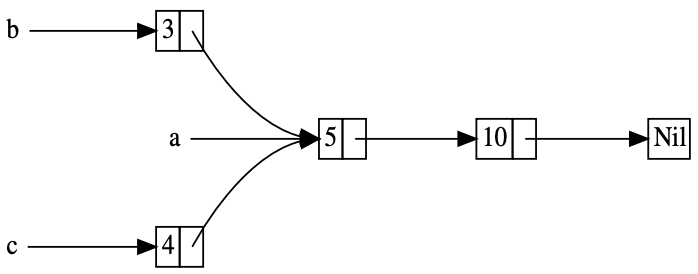
\includegraphics[width=0.9\textwidth]{img/rc.png}
\end{center}
Una prima dichiarazione errata può essere:
\begin{tcolorbox}
\begin{verbatim}
enum List {
 Cons(i32, Box<List>),
 Nil,
}

use List::{Cons, Nil};

fn main() {
 let a = Cons(5,
 Box::new(Cons(10,
 Box::new(Nil))));
 let b = Cons(3, Box::new(a));
 let c = Cons(4, Box::new(a));
}
\end{verbatim}
\end{tcolorbox}
Questo codice non compila: cosa succederebbe se \texttt{b} andasse out-of-scope e \texttt{c} no?

Una dichiarazione corretta, con smart pointer \textit{reference counting}, può essere:
\begin{tcolorbox}
\begin{verbatim}
enum List {
 Cons(i32, Rc<List>),
 Nil,
}

use List::{Cons, Nil};
use std::rc::Rc;

fn main() {
 let a = Rc::new(Cons(5, Rc::new(Cons(10, Rc::new(Nil)))));
 let b = Cons(3, Rc::clone(&a));
 let c = Cons(4, Rc::clone(&a));
}
\end{verbatim}
\end{tcolorbox}
\texttt{Rc::new} alloca spazio nello heap per un dato + il suo contatore di riferimenti.\\
\texttt{Rc::clone} incrementa il reference counter.

Quando \texttt{b} e \texttt{c} vanno out-of-scope il counter di \texttt{a} viene decrementato di 2 e, raggiunto lo 0, anche \texttt{a} viene deallocato dallo heap.

Inoltre, Rust garantisce che un dato possa avere al più una reference mutable oppure un numero arbitrario di reference in sola lettura (evitando possibili data races).\\
\texttt{Box<T>} non ha restrizioni da questo punto di vista, mentre \texttt{Rc<T>} permette solamente reference di sola lettura!

\pagebreak

\subsubsection*{RefCell<T>}
Questo smart pointer cerca di risolvere il problema di reference di sola lettura degli \texttt{Rc<T>}. E' uno smart pointer che \textbf{a runtime} verifica la condizione: \textit{al più una mutable reference o n immutable ones} (tramite un sistema di lock). In caso contrario, viene sollevato un \texttt{panic}.

Questo smart pointer va usato con parsimonia: meglio affidarsi al controllo a compile-time di Rust.

Un suo esempio di utilizzo può essere:
\begin{tcolorbox}
\begin{verbatim}
enum List {
 Cons(Rc<RefCell<i32>>, Rc<List>),
 Nil,
}
...
fn main() {
 let value = Rc::new(RefCell::new(5));
 let a = Rc::new(Cons(Rc::clone(&value), Rc::new(Nil)));
 let b = Cons(Rc::new(RefCell::new(6)), Rc::clone(&a));
 let c = Cons(Rc::new(RefCell::new(10)), Rc::clone(&a));

 *value.borrow_mut() += 10;     // per mutare la cella ne acquisisco 
                                // un lock in scrittura

 println!("a after = {:?}", a);
 println!("b after = {:?}", b);
 println!("c after = {:?}", c);
}
\end{verbatim}
\end{tcolorbox}
In questo caso, le code possono essere sharate in maniera immutabile all'interno di un solo thread, mentre le teste possono sharate e sono anche mutabili (RefCell permette di mutarle, Rc di shararle).

\subsubsection*{Weak<T>}
La tecnica del reference counting porta a memory leaks in caso di cicli. Spesso in un ciclo vi sono dei puntatori che rappresentano che sono naturalmente \textbf{forti} e altri \textbf{deboli}.

Una cella è viva quando ha almeno un puntatore forte entrante; morta altrimenti (si traduce in: i deboli non contano ai fini del reference counting).

Un possibile esempio di utilizzo è un albero. Un nodo ha:
\begin{itemize}
    \item Due puntatori forti (e.g. Rc<Node>) ai figli destro e sinistro.
    \item Un puntatore debole (Weak<Node>) al padre.
\end{itemize}

Se un nodo viene sganciato da un’albero (ovvero il padre non punta più a lui) allora diventa unreachable e deve essere eliminato.

Ma non solo: tutti i suoi discendenti sono unreacheable e vanno reclamati. Questo anche se il nodo e tutti i discendenti si puntano fra di loro (i figli puntano al padre, ma debolmente).

Lo smart pointer \texttt{Weak<T>} implementa un trait con due metodi:
\begin{itemize}
    \item \texttt{upgrade(r Weak<T>) -> Option< Rc<T> >}: data una weak reference ritorna una \texttt{Rc<T>} reference se l’oggetto è ancora allocato.
    \item \texttt{downgrade(r Rc<T>) -> Weak<T>}: restituisce un weak pointer per un \texttt{Rc<T>}.
\end{itemize}
\vspace{8pt}
Anche nei linguaggi con garbage collector si possono creare situazioni dove la memoria non viene reclamata anche se dovrebbe Ad esempio, una hash-table viene utilizzata per fare memoization, ovvero associare input a output di una funzione per non ricalcolarli.

Se il puntatore dalla hash-table all’input è strong, poiché la hash-table è sempre reachable, tutti gli input usati in passato non possono essere più reclamati anche se sono unreachable in altri modi. I weak pointers risolvono proprio questo problema.

\subsubsection*{Mutex<T> e Arc<T>}
Esistono numerosi altri smart pointers usati in scenari concorrenti con memoria condivisa, come:
\begin{itemize}
    \item \texttt{Mutex<T>}: con metodo bloccante \texttt{lock()} per ottenere reference al contenuto \texttt{T}.
    \item \texttt{Arc<T>}: reference counting \textit{atomico} da utilizzare in contesti concorrenti.
\end{itemize}
Utilizzare smart pointers per scenari concorrenti porta ovviamente ad un costo maggiore (causato dalla gestione dei lock), quindi vanno usati quanto strettamente necessari.

\subsubsection*{User defined smart pointers}
Per creare uno smart pointer definito in user space è sufficiente definire una strattura dati che implementa un certo numero di traits (a seconda di quali features delle reference volete).

Talvolta per implementare certe funzionalità è necessario fare ricorso a costrutti \textbf{unsafe} del linguaggio (che manipolano la memoria bypassando i rigidi controlli di Rust).

\pagebreak

Un possibile esempio di smart pointer definito in user space può essere:
\begin{tcolorbox}
\begin{verbatim}
struct MyBox<T>(T);     // una tupla con un solo campo

impl<T> MyBox<T> {      
 fn new(x: T) -> MyBox<T> { MyBox(x) }      // costruttore del dato
}

...

impl<T> Deref for MyBox<T> {    // implementiamo il dereferencing, *
 type Target = T;               // associated type: * restituisce un &T,
                                // ovvero una reference al Target che è T

 fn deref(&self) -> &T { &self.0 }      // il T è il valore dell’unico 
                                        // campo della tupla
}

impl<T> Drop for MyBox<T> {     // implementiamo il drop del dato
 fn drop(&mut self) {
    println!("Dropping MyBox<T> with data `{}`!", self.0);
 }
}

fn main() {
 let x = MyBox::new(4);                 // crea una smart pointer per 4
 let y = *x;                            // lo dereferenzia
 println!("x = {}, y = {}", x, y);
} // lo smart pointer esce di scope
\end{verbatim}
\end{tcolorbox}
Una possibile esecuzione di questo codice può essere:\\
\texttt{x = 4, y = 4\\
Dropping MyBox<T> with data `4`!
}

\subsection*{Alcune osservazioni finali su Rust}
L’analisi statica di Rust aiuta a prevenire moltissimi errori comuni nella gestione esplicita della memoria e nella concorrenza con memoria condivisa.

I messaggi di errore sono spesso molto complessi da decifrare e la soluzione è spesso non ovvia.

Bisogna cercare la (ri)formulazione del codice/algoritmo accettata da Rust.

Necessaria ottima conoscenza degli smart pointers di libreria.
\end{document}